\documentclass[11pt]{article}
\usepackage{amsmath}
\usepackage[utf8]{inputenc}
\usepackage{amsfonts,url,epsfig,breakurl}
%%% Document layout, margins
\usepackage{geometry} 
\geometry{letterpaper, textwidth=6.5in, textheight=9in, marginparsep=1em}
%%% Section headings
\usepackage{sectsty} 
\usepackage[normalem]{ulem}
%\setlength{\baselineskip}{40pt}

%\usepackage{hyperref}
\usepackage{todonotes}
\newcommand{\AG}[1]{\todo[inline,author=AG]{#1}}
\newcommand{\ag}[1]{\todo[size=\tiny]{ag: #1}{}}
\newcommand{\MV}[1]{\todo[inline,author=MV]{#1}}
\newcommand{\mv}[1]{\todo[size=\tiny]{mv: #1}{}}


\sectionfont{\sffamily\bfseries\upshape\large}
\subsectionfont{\sffamily\bfseries\upshape\normalsize} 
\subsubsectionfont{\sffamily\mdseries\upshape\normalsize}
\makeatletter
\renewcommand\@seccntformat[1]{\csname the#1\endcsname.\quad}
\makeatother\renewcommand{\bibitem}{\vskip2pt\par\hangindent\parindent\hskip-\parindent}
\newcommand{\mme}{\mathbb{E}}

\makeatletter
\def\@maketitle{%
  \begin{center}%
  \let \footnote \thanks
    {\large \@title \par}%
    {\normalsize
      \begin{tabular}[t]{c}%
        \@author
      \end{tabular}\par}%
    {\small \@date}%
  \end{center}%
}
\makeatother


\title{\bf Bayesian analysis of tests with unknown specificity and sensitivity\footnote{We thank the National Science Foundation, Office of Naval Research, National Institutes of Health, and Schmidt Foundation for financial support.  R and Stan code for the computations in this paper are at **.}\vspace{.1in}}

\author{Andrew Gelman\footnote{Department of Statistics and Department of 
Political Science, Columbia University, New York.}  \ and Bob Carpenter\footnote{Center for Computational Mathematics, Flatiron Institute, New York}
\vspace{.1in}}

\date{17 May 2020}

\begin{document}\sloppy
\maketitle

\begin{abstract}
When testing for a rare disease, prevalence estimates can be highly sensitive to uncertainty in the specificity and sensitivity of the test.  Bayesian inference is a natural way to propagate these uncertainties, with hierarchical modeling capturing variation in these parameters across experiments.  Another concern is the people in the sample not being representative of the general population.  Statistical adjustment cannot without strong assumptions correct for selection bias in an opt-in sample, but multilevel regression and poststratification can at least adjust for known differences between sample and population.  We demonstrate these models with code in R and Stan and discuss their application to a controversial recent study of COVID-19 antibodies in a sample of people from the Stanford University area.  Wide posterior intervals make it impossible to evaluate the quantitative claims of that study regarding the number of unreported infections.  For future studies, the methods described here should facilitate more accurate estimates of disease prevalence from imperfect tests performed on nonrepresentative samples. 
\end{abstract}

\section{Background}

Correction of diagnostic tests for false positives and false negatives is a well-known probability problem.  When the base rate is low, estimates become critically sensitive to misclassifications (Hemenway, 1997).  This issue hit the news recently with a recent study of coronavirus antibodies in a population with a low incidence rate (Bendavid et al., 2020a, Lee, 2020).

This is a problem where not fully accounting for uncertainty can make a big difference in scientific conclusions and potential policy recommendations.  In early April, 2020, Bendavid et al.\ (2020a) recruited 3330 residents of Santa Clara County, California and tested them for COVID-19 antibodies.  50 people tested positive, yielding a raw estimate of 1.5\%.  After corrections, Bendavid et al.\ (2020a) reported an uncertainty range of 2.5\% to 4.2\%, implying that the number of infections in the county was between 50 and 85 times the count of cases reported at the time.  Using an estimate of the number of coronavirus deaths in the county up to that time, they computed an implied infection fatality rate (IFR) of 0.12--0.2\%, much lower than IFRs in the range of 0.5\%--1\% that had been estimated from areas with outbreaks of the disease.

The estimates from Bendavid et al.\ (2020a) were controversial, and it turned out that they did not correctly account for uncertainty in the specificity (true positive rate) of the test.  There was also concern about the adjustment they performed for nonrepresentativeness of their sample.  Thus, the controversy arose from statistical adjustment and assessment of uncertainty.  In the present article we set up a Bayesian framework to clarify these issues, setting up and fitting models using the probabilistic programming language Stan (Stan Development Team, 2020).


\section{Modeling a test with uncertain sensitivity and specificity}\label{model1}

Testing for a rare disease is a standard textbook example of conditional probability, famous for the following counterintuitive result:  Suppose a person tests positive for a disease, based on a test that has a 95\% accuracy rate, and further suppose that this person is sampled at ramdom from a population with a 1\% prevalence rate.  Then what is the probability that he or she actually has the disease? The usual intuition suggests that the conditional probability should be approximately 95\%, but it is actually, as can be seen from a simple calculation of base rates, as suggested by Gigerenzer et al.\ (2007).  Imagine you test 1000  people:  with a 1\% prevalence rate, we can expect that 10 have the disease and 990 do not.  Then, given the assumed 95\% accuracy rate (assuming this applies to both specificity and sensitivity of the test), we would expect $0.95*10=9.5$ true positives and $0.05*990 =  49.5$ false positives; thus, the proportion of positive tests that are true positives is $9.5/(9.5+49.5) = 0.16$, a number that is difficult to make sense of without visualizing the hypothetical populations of true positive and false positive tests.

A related problem is to take the rate of positive tests and use it to estimate the prevalence of the disease.  If the population prevalence is $\pi$ and the test has a specificity of $\gamma$ and a sensitivity of $\delta$, then the expected frequency of positive tests is $p=(1-\gamma)(1- \pi)+ \delta\pi$.  So, given known $\gamma$, $\delta$ and $p$, we can solve for the prevalence,
\begin{equation}\label{solve}
  \pi=(p + \gamma - 1)/(\delta + \gamma - 1).
  \end{equation}
  If the properties of the test are known, but $p$ is estimated from a random sample, we can obtain a simple classical estimate by starting with a confidence interval for $p$ and then propagating it through the formula  For example, Bendavid et al.\ (2020) report 50 positive tests out of 3330, which corresponds to an estimate  $\hat{p}=50/3000=0.015$ with standard error $\sqrt{0.015(1-0.015)/3330}=0.002$.  Supposing that their test had a specificity of $\gamma=0.995$ and a sensitivity of $\delta=0.80$, this yields an estimate of $(0.015 + 0.995 - 1)/(0.80 + 0.995 -1) = 0.013$ with standard error $0.002/(0.80 + 0.995 -1) = 0.003$.

 Two immediate difficulties arise with the classical approach.  First, if the observed rate $\hat{p}$ is less than  $1-\gamma$, the false positive rate of the test, then the estimate from (\ref{solve}) becomes meaninglessly negative.  Second, if there is uncertainty in the specificity and sensitivity parameters, it becomes challenging to propagate uncertainty through the nonlinear expression (\ref{solve}).

We can resolve both these problems with a simple Bayesian analysis.

First, suppose that estimates and uncertainties for sensitivity and specificity have been externally supplied.  The model is then:
\begin{align}
\nonumber  y & \sim \mbox{Binomial} (n, p)\\
\nonumber   p & = (1-\gamma)(1- \pi)+ \delta\pi\\
\nonumber  \gamma & \sim \mbox{normal}(\mu_{\gamma}, \sigma_{\rm gamma})\\
\label{normals}  \delta & \sim \mbox{normal}(\mu_{\delta}, \sigma_{\rm delta}),
\end{align}
and Stan code is given in Appendix \ref{stan1}.
For simplicity, we have used independent normal prior distributions (with the constraint that both parameters are restricted to the unit interval), but it would be easy enough to use other distributions if prior information were available in that form.

In the example of Bendavid (2020a), prior information on specificity and sensitivity was given in the form of previous trials, yielding the model,
  \begin{align*}
   y & \sim \mbox{Binomial} (n, p)\\
  p & = (1-\gamma)(1- \pi)+ \delta\pi\\
   y_{\gamma} & \sim \mbox{Binomial} (n_{\gamma}, \gamma)\\
   y_{\delta} & \sim \mbox{Binomial} (n_{\delta}, p_{\delta}).
 \end{align*}
 Fitting this model given the data in that report ($y_{\rm gamma}/n_{\gamma}=399/401$ and $y_{\rm delta}/n_{\delta}=103/122$) yields a wide uncertainty for $p$.  Stan code is in Appendix \ref{stan2}.

 \begin{figure}
\centerline{ 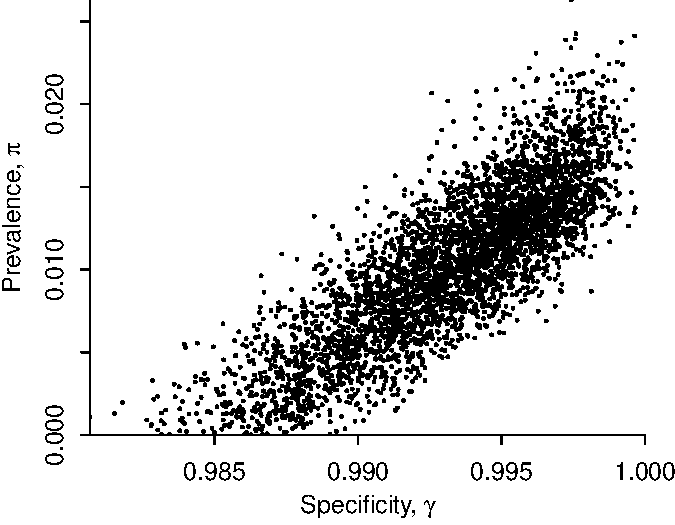
\includegraphics[width=.45\textwidth]{scatter.pdf} 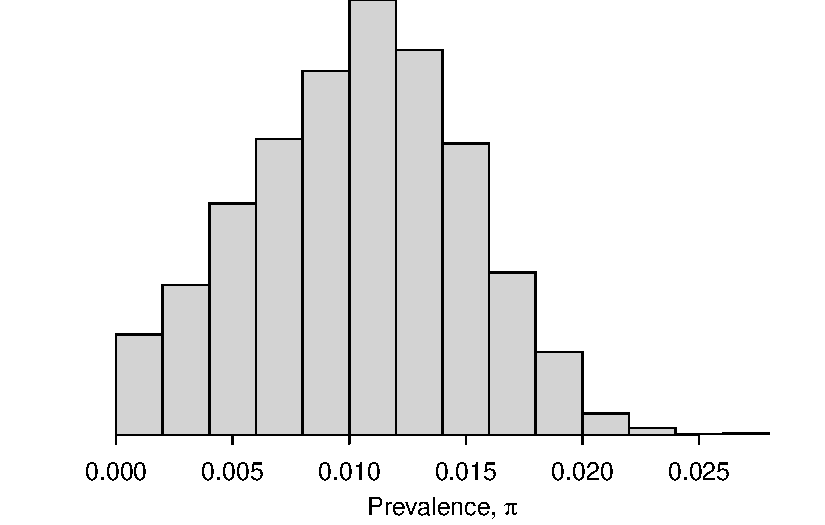
\includegraphics[width=.55\textwidth]{hist.pdf}}
\caption{\em Summary of inference from model with unknown specificity, sensitivity, and prevalence, based on data from Bendavid et al.\ (2020a):  (a) scatterplot of posterior simulations of prevalence, $\pi$, and specificity, $\gamma$; (b) histogram of posterior simulations of $\gamma$.}
\label{posterior1}
\end{figure} 

Figure \ref{posterior1}a shows the joint posterior simulations for $p$ and $\gamma$:  uncertainty in the population prevalence is in large part driven by uncertainty in the specificity.  Figure \ref{posterior1}b shows the posterior distribution for $p$, which reveals that the data and model are consistent with prevalences as low as 0 and as high as nearly 2\%.

The asymmetric posterior distribution with its hard bound at zero suggests that the usual central 95\% interval will not be a good inferential summary.  Instead we use highest posterior density or shortest posterior interval, for reasons discussed in Liu, Gelman, and Zheng (2015). The resulting 95\% interval for $\pi$ is (0, 1.8\%), which is much different from the interval (1.1\%, 2.0\%) reported by Bendavid et al.\ (2020a).  As a result, the substantive conclusion from that earlier report has been overturned. From the given data, the uncertainty in the specificity is large enough that the data do not supply strong evidence of a substantial prevalence.

\section{Hierarchical model for varying testing conditions}\label{model2}
The above analysis reveals that inference about specificity is key to precise estimation of low prevalence rates.  In the second version of their report, Bendavid et al.\ (2020b) include data from 13 specificity studies and 3 sensitivity studies.  Sensitivity and specificity can vary across experiments, so it is not appropriate to simply pool the data from these separate studies.  Instead, we set up a hierarchical model where, for any study $j$, the specificity $\gamma_j$ and sensitivity $\delta_j$ are drawn from normal distributions on the logistic scale,
\begin{align*}
  \mbox{logit}(\gamma_j) & \sim \mbox{normal}(\mu_{\gamma}, \sigma_{\rm gamma})\\
 \mbox{logit}(\delta_j) & \sim \mbox{normal}(\mu_{\delta}, \sigma_{\rm delta}).
\end{align*}
Stan code is given in Appendix \ref{stan3}.
This is different from model (\ref{normals}) in that, with data from multiple calibration studies, the hyperparameters $\mu$ and $\sigma$ can be estimated from the data.  In general it could make sense to allow correlation between $\gamma_j$ and $\delta_j$ (Guo, Riebler, and Rue, 2017), but the way the data are currently available to us, specificity and sensitivity are estimated from separate studies and so there is no information about such a correlation.  When coding the model, we use the convention that $j=1$ corresponds to the study of interest, with other $j$'s representing studies of specificity and sensitivity given known samples.

We can also think more about the logistic transform, which allows the unbounded normal distribution to map to the unit interval but might not be appropriate for tests where the specificity can actually reach the value of 1.  Again, we would only expect these sorts of boundary issues to be important when the underlying prevalence is close to zero.

\begin{figure}
 \begin{small}
  \centerline{
    \begin{tabular}{l ccc c ccc}
      & \multicolumn{3}{c}{Posterior quantiles} && \multicolumn{3}{c}{Posterior quantiles} \\
      & \multicolumn{3}{c}{with weak prior} && \multicolumn{3}{c}{with stronger prior} \\
     Parameter & 2.5\% & median & 97.5\% && 2.5\% & median & 97.5\% \\\hline
     Prevalence, $\pi$ & 0.003 & 0.017 & 0.354 && 0.003 & 0.012 & 0.021 \\
     Specificity, $\gamma_1$ & 0.986 & 0.998 & 1.000 && 0.988 & 0.995 & 0.998 \\
     Sensitivity, $\delta_1$ & 0.031 & 0.757 & 0.973 && 0.642 & 0.818 & 0.910 \\
     $\mu_{\gamma}$ & 4.63 & 5.69 & 7.20 && 4.71 & 5.26 & 5.87 \\
     $\mu_{\delta}$ & $\!\!\!\!\!-0.55$ & 1.36 & 2.64 && 0.94 & 1.51 & 2.06 \\
     $\sigma_{\gamma}$ & 0.89 & 1.66 & 2.78 && 0.04 & 0.42 & 0.77 \\ 
     $\sigma_{\delta}$ & 0.22 & 0.90 & 2.32 && 0.02 & 0.26 & 0.57
  \end{tabular}
}
\end{small}
  \caption{\em Summary of inferences for the prevalence, specificity, and sensitivity of the Bendavid et al.\ (2020b) experiment, along with inferences for the hyperparameters characterizing the distribution of specificity and sensitivity on the logistic scale.  (a) For the model with weak priors for $\sigma_{\gamma}$ and $\sigma_{\delta}$, the posterior inference for the prevalence, $\pi$, is highly uncertain.  This is driven by the wide uncertainty for the sensitivity, which is driven by the large uncertainty in the hyperparameters for the sensitivity distribution. (b) Stronger priors on  $\sigma_{\gamma}$ and $\sigma_{\delta}$ have the effect of regularizing the specificity and sensitivity parameters, leading to narrower intervals for $\pi$, the parameter of interest in this study.  The hyperparameters $\mu$ and $\sigma$ are on the logistic scale so are difficult to interpret without transformation.}
\label{posterior2}
\end{figure} 

We first fit the above model to the data from Bendavid et al.\ (2020b), with weak $\mbox{normal}(0,1)$ priors on $\sigma_{\gamma}$ and $\sigma_{\delta}$.  The results are shown in Figure \ref{posterior2}a.  The 95\% posterior interval for the prevalence is now $(0.00, 0.19)$.  Where does that upper bound come from:  how could an underlying prevalence of 19\% be possible, given that only 1.5\% of the people in the sample tested positive?  The answer can be seen from the huge uncertainty in the sensitivity parameter, which in turn comes from the possibility that $\sigma_{\delta}$ is very large.  The trouble is that the sensitivity information in these data comes from only 3 experiments, which is not enough to get a good estimate of the underlying distribution.  This is a problem discussed by Guo, Riebler, and Rue (2017).

The only way to make progress here is to constrain the sensitivity parameters in some way.  One possible strong assumption is to assume that $\sigma_{\delta}$ is some small value. In the current context, it makes sense to consider this assumption, as we can consider it a relaxation of the assumption of Bendavid et al.\ (2020b) that $\sigma_{\delta} = 0$.  We also have reason to believe that specificity will not vary much between experiments, so we will apply a soft constraint to the variation in specificities as well.

We replace the weakly informative $\mbox{normal}^+(0, 1)$ priors on $\sigma_{\gamma}$ and $\sigma_{\delta}$ with something stronger, 
$\sigma_{\gamma}, \sigma_{\delta}\sim\mbox{normal}^+(0, 0.2)$.  To get a sense of what this means, start with the point estimate from Figure \ref{posterior2}a of $\mu_{\delta}$, which is 1.36. Combining with this new prior implies that there's a roughly 2/3 chance that the sensitivity of the assay in a new experiment is in the range $\mbox{logit}^{-1}(1.36 \pm 0.2)$, which is $(0.76, 0.83)$. This seems reasonable.

Figure \ref{posterior2}b shows the results.  Our 95\% interval for $\pi$ is now $(0.003, 0.021)$, that is, the estimated infection rate is estimated to be somewhere between 0.3\% and 2.1\%.


 \section{Extensions of the model}

\subsection{Multilevel regression and poststratification to adjust for differences between sample and population}\label{mrp}

Bendavid et al.\ compared demographics on 3330 people they tested, and they found differences in the distributions of sex, age, ethnicity, and zip code of residence compared to the general population of Santa Clara County. It would be impossible to poststratify the raw data on 2 sexes, 4 ethnicity categories,  4 age categories, and 58 zip codes, as the resulting 1856 cells would greatly outnumber the positive tests in the data.  Bendavid (2020a,b) adjusted for sex $\times$ ethnicity $\times$ zip code, but their analysis is questionable, first because they did not adjust for age, and second because of noisy weights arising from the variables they did adjust for.
To obtain stable estimates while adjusting for all these variables, we would recommend applying a multilevel model to the exposure probability, thus replacing the constant $\pi$ in the above models with something like this logistic regression:
\begin{equation*}
\pi_i = \mbox{logit}^{-1}(\beta_1 + \beta_2*\rm{male} + \beta_3*x^{\rm zip}_{\rm zip[i]} + \alpha^{\rm eth}_{\rm eth[i]} + \alpha^{\rm age}_{\rm age[i]} + \alpha^{\rm zip}_{\rm zip[i]}),
\end{equation*}
where male is a variable that takes on the value $-0.5$ for women $+0.5$ for men; $x^{\rm zip}$ is a relevant predictor at the zip code level; eth[i], age[i], and zip[i] are index variables for the survey respondents $i$; the $\beta$'s are logistic regression coefficients, and the $\alpha$'s are vectors of varying intercepts:
\begin{align*}
  \alpha^{\rm name} &\sim \mbox{normal}(0, \sigma_{\rm name}),\mbox{ for } \mbox{name} = \mbox{eth, age, zip}.
\end{align*}
It will be important to include the predictor $x^{\rm zip}$, which in this example might be percent Latino or average income in the zip code.  Otherwise, with so many zip codes, the multilevel model will just partially pool most of the zip code adjustments to zero, and not much will be gained from the geographic poststratification.

The above model is a start; it coud be improved by including interactions, following the general ideas of Ghitza and Gelman (2013),  In any case, once this model has been fit, it can be used to make inferences for disease prevalence for all cells in the population, and these cell estimates can then be summed, weighting by known population totals (in this case, the number of people in each sex $\times$ ethnicity $\times$ age $\times$ zip code category in the population) to get inferences for the prevalence in the county.  Here we are implicitly assuming that the data represent a random sample within poststratification cells.

In addition, priors are needed for $\sigma_{\rm eth}, \sigma_{\rm age},\sigma_{\rm zip}$, and $\beta$, along with the hierarchical specificity and sensitivity parameters from the earlier model.

We coded this model in Stan (see Appendix \ref{stan4}).  Unfortunately the raw data from Bendavid et al.\  are not currently available, so we fit the model to simulated data to check the stability of the computation.  We used a $\mbox{normal}(0,2.5)$ prior for $\beta_1$ (corresponding to an approximate 95\% prior interval of $(0.7\%, 99.3\%)$ for the prevalence), a $\mbox{normal}(0,0.5)$ prior for $\beta_2$, and $\mbox{normal}^+(0, 0.5)$ priors for $\sigma_{\rm eth}, \sigma_{\rm age},\sigma_{\rm zip}$.  These priors allow the prevalence to vary moderately by these poststratification variables.

Once the above model has been fit, it implies inferences for the prevalence in each of the $2\times 4 \times 4 \times 58$ poststratification cells, and these can be averaged to get a population prevalence:  $p_{\rm avg} = \sum_jN_jp_j/\sum_jN_j$, where $N_j$ is the number of people in cell $j$ in the general population, and $p_i$ is the prevalence as computed from the logistic model.  We perform this summation in the generated quantities block of the Stan model in Appendix \ref{stan4}.

\subsection{Variation across location and over time}\label{muiltiple}
The aforementioned Santa Clara County study is just one of many recent COVID-19 antibody surveys.  Other early studies were conducted in Boston, New York, Los Angeles, and Miami, and in many places outside the United States, and we can expect many more in the future.  If the raw data from these studies were combined, it should be possible to estimate the underlying prevalences from all these studies using a hierarchical model, allowing specificity, sensitivity, and prevalence to vary by location.  Such an analysis is performed by Levesque and Maybury (2020) using detailed information on the different tests used in different studies.

We will also be seeing more studies of changing infection rates over time.  Stringhini et al.\ (2020) perform usch an analysis of weekly surveys in Geneva, Switzerland, accounting for specificity and sensitivity and poststratifying by sex and age.

\section{Non-Bayesian approaches}
As with any statistical analysis, alternative approaches are possible that would give similar results.

In Section \ref{model1}, it was necessary to (a) account for uncertainty in all three parameters and (b) respect the constraint that all three probabilities had to be between 0 and 1.  We assume that both these aspects of the model could have been incorporated into a non-Bayesian approach by working out the region in the space of $(\pi,\gamma,\delta)$ that was consistent with the data and then constructing a family of tests which could be inverted to create confidence regions.

This could be expanded into a multilevel model as in Section \ref{model2} by considering the specificities and sensitivities of the different experiments as missing data and averaging over their distribution, but still applying non-Bayesian inference to the resulting hyperparameters.  The wide uncertainty intervals from the analysis in Section \ref{model2} suggest that some constraints or regularization or additional information on the hyperparameters would be necessary to get stable inferences here, no matter what statistical approach is used.

Finally, some rough equivalent to the poststratification adjustment in Section \ref{mrp} could be performed using a non-Bayesian weighting approach, using some smoothing to avoid the noisiness of raw poststratification weights.  Similarly, non-Bayesian methods could be used to fit regressions allowing prevalence to vary over location and time.

\section{Discussion}


\subsection{Limitations of the statistical analysis}


Epidemiology in general, and disease testing in particular, features latent parameters with high levels of uncertainty, difficulty in measurement, and uncertainty about the measurement process as well.  This is the sort of setting where it makes sense to combine information from multiple studies, using Bayesian inference and hierarchical models, and where inferences can be sensitive to assumptions.

The biggest assumptions in this analysis are, first, that the historical specificity and sensitivity data are relevant to the current experiment; and, second, that the people in the study are a representative sample of the general population.  We addressed the first concern with a hierarchical model of varying sensitivities and specificities, and we addressed the second concern with multilevel regression and poststratification on demographics and geography.  But this modeling can take us only so far.  If there is hope or concern that the current experiment is has unusual measurement properties, or that the sample is unrepresentative in ways not accounted for in the regression, then more information or assumptions need to be included in the model.

The other issue is that there are choices of models, and tuning parameters within each model.  Sensitivity to the model is apparent in Bayesian inference, but it would arise with any other statistical method as well.  For example, Bendavid et al.\ (2020a) used an (incorrectly applied) delta method to propagate uncertainty, but this is problematic when sample size is low and probabilities are near 0 or 1.  Bendavid  et al.\ (2020b) completely pooled their specificity and sensitivity experiments, which is equivalent to setting $\sigma_{\gamma}$ and $\sigma_{\delta}$ to zero.  And their weighting adjustment has many arbitrary choices.  We note these not to single out these particular authors but rather to emphasize that, at least for this problem, all statistical inferences involve user-defined settings.

For the models in the present article, the most important user choices are:  (a) what data to include in the analysis, (b) prior distributions for the hyperparameters, and (c) the structure and interactions to include in the MRP model.  For these reasons, it would be difficult to set up the model as a plug-and-play system where users can just enter their data, push a button, and get inferences.  Some active participation in the modeling process is required, which makes sense given the sparseness of the data.  When studying populations with higher prevalences and with data that are closer to random samples, more automatic approaches might be possible.

\subsection{Santa Clara study}

Section \ref{model2} shows our inferences given the summary data in Bendavid et al.\ (2020b).
The inference depends strongly on the priors on the distributions of sensitivity and specificity, but that is unavoidable:  the only way to avoid this influence of the prior would be to sweep it under the rug, for example by just assuming a zero variation in the test parameters.

What about the claims regarding the rate of coronavirus exposure and implications for the infection fatality rate?  It's hard to say from this one study:  the numbers in the data are consistent with zero infection rate and a wide variation in specificity and sensitivity across tests, and the numbers are also consistent with the claims made in Bendavid et al.\ (2020a,b). That does not mean anyone thinks the true infection rate is zero.  It just means that more data, assumptions, and subject-matter knowledge are required. That's ok---people usually make lots of assumptions in this sort of laboratory assay. It's common practice to use the manufacturer's numbers on specificity, sensitivity, detection limit, and so forth, and not worry about that level of variation. It's only when you are estimating a very low underlying rate that the statistical challenges become so severe.

One way to go beyond the ideas of this paper would be to include additional information on patients, for example from self-reported symptoms.  Some such data are reported in Bendavid et al.\ (2020b), although not at the individual level. With individual-level symptom and test data, a model with multiple outcomes which could yield substantial gains in efficiency compared to the existing analysis using only the positive/negative test result.

For now, we do not think the data support the claim that the number of infections in Santa Clara County was between  50 and 85 times the count of cases reported at the time, or the implied interval for the IFR of 0.12--0.2\%.  These numbers are consistent with the data, but the data are also consistent with a near-zero infection rate in the county.  The data of Bendavid et al.\ (2020a,b) do not provide strong evidence about the number of people infected or the infection fatality ratio; the number of positive tests in the data is just too small, given uncertainty in the specificity of the test.

Going forward, the analyses in this article suggest that future studies should be conducted with full awareness of the challenges of measuring specificity and sensitivity, that relevant variables be collected on study participants to allow inference for the general population, and that (de-identified) data be accessible to external researchers.


\section*{References}

\noindent

\bibitem  Bendavid, E., Mulaney, B., Sood, N., Shah, S., Ling, E., Bromley-Dulfano, R., Lai, C.,  Weissberg, Z., Saavedra-Walker, R., Tedrow, J., Tversky, D., Bogan, A., Kupiec, T., Eichner, D., Gupta, R., Ioannidis, J., and Bhattacharya, J. (2020a).  COVID-19 antibody seroprevalence in Santa Clara County, California, version 1. \url{https://www.medrxiv.org/content/10.1101/2020.04.14.20062463v1.full.pdf}

\bibitem  Bendavid, E., Mulaney, B., Sood, N., Shah, S., Ling, E., Bromley-Dulfano, R., Lai, C.,  Weissberg, Z., Saavedra-Walker, R., Tedrow, J., Tversky, D., Bogan, A., Kupiec, T., Eichner, D., Gupta, R., Ioannidis, J., and Bhattacharya, J. (2020b).  COVID-19 antibody seroprevalence in Santa Clara County, California, version 2. \url{https://www.medrxiv.org/content/10.1101/2020.04.14.20062463v2.full.pdf}

\bibitem Gelman, A. (2020).  Simple Bayesian analysis inference of coronavirus infection rate from the Stanford study in Santa Clara county. {\em Statistical Modeling, Causal Inference, and Social Science}, 1 May.  \url{https://statmodeling.stat.columbia.edu/2020/05/01/simple-bayesian-analysis-inference-of-coronavirus-infection-rate-from-the-} \url{stanford-study-in-santa-clara-county}

\bibitem Ghitza, Y., and Gelman, A., (2013). Deep interactions with MRP: Election turnout and voting patterns among small electoral subgroups. {\em American Journal of Political Science} {\bf 57}, 762--776. 
  
\bibitem Gigerenzer, G., Gaissmaier, W., Kurz-Milcke, E., Schwartz, L. M., and Woloshin, S.  (2007).  Helping doctors and patients make sense of health statistics.  {\em Psychological Science in the Public Interest} {\bf 8}, 53--96.

\bibitem Guo, J., Riebler, A., and Rue, H. (2017).  Bayesian bivariate meta-analysis of diagnostic test studies with interpretable priors.  {\em Statistics in Medicine} {\bf 36}, 3039--3058.

\bibitem Hemenway, D. (1997).  The myth of millions of annual self-defense gun uses:  A case study of survey overestimates of rare events.  {\em Chance} {\bf 10} (3), 6--10.

\bibitem Lee, S. M. (2020).  Two antibody studies say coronavirus infections are more common than we think. Scientists are mad.  {\em BuzzFeed News}, 22 Apr.  \url{https://www.buzzfeednews.com/article/stephaniemlee/coronavirus-antibody-test-santa-clara-los-angeles-stanford}

\bibitem Levesque, J., and Maybury, D. W. (2020).  A note on COVID-19 seroprevalence studies: a meta-analysis using hierarchical modelling.  \url{https://www.medrxiv.org/content/10.1101/2020.05.03.20089201v1.full.pdf}

\bibitem Liu, Y., Gelman, A., and Zheng, T. (2015).  Simulation-efficient shortest probability intervals. {\em Statistics and Computing} {\bf 25}, 809--819.

\bibitem Stan Development Team (2020). {\em Stan Modeling Language User's Guide and Reference Manual}.  \url{https://mc-stan.org}

\bibitem Stringhini, S., Wisniak, A., Piumatti, G., Azman, A. S., Lauer, S. A., Baysson, H., De Ridder, D., Petrovic, D.,  Schrempft, S., Marcus, K., Yerly, S., Vernez, I. A., Keiser, O., Hurst, S., Posfay-Barbe, K. M., Trono, D., Pittet, D., Getaz, L., Chappuis, F., Eckerle, I., Vuilleumier, N., Meyer, B., Flahault, A., Kaiser, L., and Guessous, I. (2020).  Repeated seroprevalence of anti-SARS-CoV-2 IgG antibodies in a population-based sample.  \url{https://www.medrxiv.org/content/10.1101/2020.05.02.20088898v1.full.pdf}

  \appendix

  \section{Stan programs}

  \subsection{Model with truncated normal priors on specificity and sensitivity}\label{stan1}

  \begin{small}
  \begin{quotation}\noindent
\begin{verbatim}
data {
  int y_sample;
  int n_sample;
  real mu_spec;
  real<lower=0> sigma_spec;
  real mu_sens;
  real<lower=0> sigma_sens;
}
parameters {
  real<lower = 0, upper = 1> p;
  real<lower = 0, upper = 1> spec;
  real<lower = 0, upper = 1> sens;
}
model {
  real p_sample;
  p_sample = p * sens + (1 - p) * (1 - spec);
  y_sample ~ binomial(n_sample, p_sample);
  spec ~ normal(mu_spec, sigma_spec);
  sens ~ normal(mu_sens, sigma_sens);
}
\end{verbatim}
\end{quotation}
\end{small}

  \subsection{Model with binomial data on specificity and sensitivity}\label{stan2}

    \begin{small}
  \begin{quotation}\noindent
\begin{verbatim}
data {
  int y_sample;
  int n_sample;
  int y_spec;
  int n_spec;
  int y_sens;
  int n_sens;
}
parameters {
  real<lower=0, upper=1> p;
  real<lower=0, upper=1> spec;
  real<lower=0, upper=1> sens;
}
model {
  real p_sample;
  p_sample = p * sens + (1 - p) * (1 - spec);
  y_sample ~ binomial(n_sample, p_sample);
  y_spec ~ binomial(n_spec, spec);
  y_sens ~ binomial(n_sens, sens);
}
\end{verbatim}
\end{quotation}
\end{small}
  
\subsection{Hierarchical model for specificities and sensitivities}\label{stan3}

  \begin{small}
  \begin{quotation}\noindent
\begin{verbatim}
data {
  int y_sample;
  int n_sample;
  int J_spec;
  int y_spec [J_spec];
  int n_spec [J_spec];
  int J_sens;
  int y_sens [J_sens];
  int n_sens [J_sens];
  real logit_spec_prior_scale;
  real logit_sens_prior_scale;
}
parameters {
  real<lower=0,upper=1> p;
  real mu_logit_spec;
  real mu_logit_sens;
  real<lower=0> sigma_logit_spec;
  real<lower=0> sigma_logit_sens;
  vector<offset=mu_logit_spec, multiplier=sigma_logit_spec>[J_spec] logit_spec;
  vector<offset=mu_logit_sens, multiplier=sigma_logit_sens>[J_sens] logit_sens;
}
transformed parameters {
  vector[J_spec] spec;
  vector[J_sens] sens;
  spec = inv_logit(logit_spec);
  sens = inv_logit(logit_sens);
}
model {
  real p_sample;
  p_sample = p*sens[1] + (1-p)*(1-spec[1]);
  y_sample ~ binomial(n_sample, p_sample);
  y_spec ~ binomial(n_spec, spec);
  y_sens ~ binomial(n_sens, sens);
  logit_spec ~ normal(mu_logit_spec, sigma_logit_spec);
  logit_sens ~ normal(mu_logit_sens, sigma_logit_sens);
  sigma_logit_spec ~ normal(0, logit_spec_prior_scale);
  sigma_logit_sens ~ normal(0, logit_sens_prior_scale);
}
\end{verbatim}
\end{quotation}
\end{small}

\subsection{Multilevel regression and poststratification}\label{stan4}

  \begin{small}
  \begin{quotation}\noindent
\begin{verbatim}
data {
  int N;                // number of tests in the sample (3330 for Santa Clara)
  int y[N];             // 1 if positive, 0 if negative
  vector[N] male;       // -0.5 if female, 0.5 if male
  int eth[N];           // 1=white, 2=asian, 3=hispanic, 4=other
  int age[N];           // 1=0-4, 2=5-18, 3=19-64, 4=65+
  int zip[N];           // zip codes 1 through 58
  int N_zip;            // number of zip codes (58 in htis case)
  vector[N_zip] x_zip;  // predictors at the zip code level
  int J_spec;
  int y_spec [J_spec];
  int n_spec [J_spec];
  int J_sens;
  int y_sens [J_sens];
  int n_sens [J_sens];
  int J;                // number of population cells, J = 2*4*4*58
  vector[J] N_pop;      // population sizes for poststratification
  real intercept_prior_mean;
  real intercept_prior_scale;
  real coef_prior_scale;
  real logit_spec_prior_scale;
  real logit_sens_prior_scale;
}
parameters {
  real mu_logit_spec;
  real mu_logit_sens;
  real<lower=0> sigma_logit_spec;
  real<lower=0> sigma_logit_sens;
  vector<offset=mu_logit_spec, multiplier=sigma_logit_spec>[J_spec] logit_spec;
  vector<offset=mu_logit_sens, multiplier=sigma_logit_sens>[J_sens] logit_sens;
  vector[3] b;           // intercept, coef for male, and coef for x_zip
  real<lower=0> sigma_eth;
  real<lower=0> sigma_age;
  real<lower=0> sigma_zip;
  vector<multiplier=sigma_eth>[4] a_eth;     // varying intercepts for ethnicity
  vector<multiplier=sigma_age>[4] a_age;     // varying intercepts for age category
  vector<multiplier=sigma_zip>[58] a_zip;    // varying intercepts for zip code
}
transformed parameters {
  vector[J_spec] spec;
  vector[J_sens] sens;
  spec = inv_logit(logit_spec);
  sens = inv_logit(logit_sens);
}
model {
  vector[N] p;
  vector[N] p_sample;
  p = inv_logit(b[1] + b[2]*male + b[3]*x_zip[zip] + a_eth[eth] + a_age[age] + a_zip[zip]);
  p_sample = p*sens[1] + (1-p)*(1-spec[1]);
  y ~ bernoulli(p_sample);
  y_spec ~ binomial(n_spec, spec);
  y_sens ~ binomial(n_sens, sens);
  logit_spec ~ normal(mu_logit_spec, sigma_logit_spec);
  logit_sens ~ normal(mu_logit_sens, sigma_logit_sens);
  sigma_logit_spec ~ normal(0, logit_spec_prior_scale);
  sigma_logit_sens ~ normal(0, logit_sens_prior_scale);
  a_eth ~ normal(0, sigma_eth);
  a_age ~ normal(0, sigma_age);
  a_zip ~ normal(0, sigma_zip);
  b[1] + b[2]*mean(male) + b[3]*mean(x_zip) ~
    normal(intercept_prior_mean, intercept_prior_scale); // prior on centered intercept
  {b[2], sigma_eth, sigma_age, sigma_zip} ~ normal(0, coef_prior_scale);
  b[3] ~ normal(0, coef_prior_scale/sd(x_zip));   // prior on scaled coefficient
}
generated quantities {
  real p_avg;
  vector[J] p_pop;        // population prevalence in the J poststratification cells
  int count;
  count = 0;
  for (i_zip in 1:58){
    for (i_age in 1:4){
      for (i_eth in 1:4){
        for (i_male in 0:1){
          count = count + 1;
          p_pop[count] = inv_logit(b[1] + b[2]*(i_male - 0.5) + b[3]*x_zip[i_zip] +
                                   a_eth[i_eth] + a_age[i_age] + a_zip[i_zip]);      
        }
      }
    }
  }
  p_avg = sum(N_pop.*p_pop)/sum(N_pop);
}
\end{verbatim}
\end{quotation}
\end{small}

\end{document}
